\documentclass[portrait,a0,final]{a0poster} % a0poster class sets the paper size
\usepackage[utf8]{inputenc}
\usepackage{microtype}
\usepackage[english]{babel}
\usepackage[pdftex]{graphicx}
\usepackage[ELEC,RGB,Uncoated]{aaltologo} % RGB, Coated, Uncoated
\usepackage{lipsum} % Lorem ipsum generator
\usepackage{verbatim} % For multiline comments

\usepackage{titlesec} % For changing the font on chapters, sections, etc.

% Math and so on
\usepackage{amsmath,amsthm,amsfonts,amssymb}
\usepackage{commath}
\usepackage{enumitem}
% TIKZ

\usepackage{tikz}
\usepackage{pgfplots}
\usepackage{color}
% and optionally (as of Pgfplots 1.3):
\pgfplotsset{compat=newest}
\pgfplotsset{plot coordinates/math parser=false}
%% Uniform lengths to use in figures
\newlength{\hfigwidth}
\setlength{\hfigwidth}{0.6\linewidth}
\newlength{\figwidth}
\setlength{\figwidth}{\linewidth}

\usetikzlibrary{decorations}
\usetikzlibrary{decorations.markings}

%% Some color definitions

\definecolor{myred}{rgb}{0.82, 0.1, 0.26} % Red
\definecolor{mygreen}{rgb}{0.0, 0.7, 0.0} % Green
\definecolor{myblue}{rgb}{0,0.4,1} % Blue
\definecolor{myyellow}{rgb}{1,0.8,0.4} % Yellowish
\definecolor{mybrown}{RGB}{169,94,43} % Brown
\definecolor{mycyan}{RGB}{29,202,190} % Cyan
\definecolor{myviolet}{RGB}{223,133,223} % Violet
\definecolor{mygreen2}{RGB}{153,230,93} % Second kind of green

\definecolor{mypink}{RGB}{102,0,204} % Pink
\definecolor{myyellow2}{RGB}{204,102,0} % Yellow

%%%% Some commands for covariance, variance and expectation done in a convenient way

%%%% MISC

% Allow page breaks inside align environments
\allowdisplaybreaks

% to prevent \u8 errors
\DeclareUnicodeCharacter{00A0}{ } 

\renewcommand{\theenumi}{(\arabic{enumi})}
% Redefine some numbering symbols
\renewcommand{\labelenumi}{\theenumi}

%%%% NEWCOMMANDS

%%% Misc

\newcommand{\bigO}{\mathcal{O}} % Asymptotic notation

%%% Functions

\DeclareMathOperator*{\argmin}{arg\,min}  % Argmin
\DeclareMathOperator*{\argmax}{arg\,max}  % Argmax

\DeclareMathOperator\erf{erf} % Standard error function

%%% Probability

\newcommand{\expec}{\mathbb{E}}           % Expectation
\newcommand{\cov}{\operatorname{Cov}}     % Covariance
\newcommand{\var}{\operatorname{Var}}     % Variance
\newcommand{\gauss}{\mathcal{N}}          % Gaussian distribution

%%% Redefine some Greeks

\renewcommand{\epsilon}{\varepsilon}

%%% Number sets

\newcommand{\R}{\mathbb{R}} % Set of real numbers
\newcommand{\Q}{\mathbb{Q}} % Set of rational numbers
\newcommand{\N}{\mathbb{N}} % Set of natural numbers
\newcommand{\Z}{\mathbb{Z}} % Set of integers

%%% Standard constants and objects
\DeclareMathOperator{\neper}{e} % Exponential constant

%% Linear algebra operations
\newcommand{\transpose}{\mathsf{T}}         % Transpose of a matrix
\newcommand{\trace}{\operatorname{tr}}      % Matrix trace
\newcommand{\adj}{\operatorname{adj}}       % Matrix adjugate
\newcommand{\diag}{\operatorname{diag}}     % Diagonal matrix
\newcommand{\rank}{\operatorname{rank}}     % rank of a matrix
\newcommand{\Hess}{\operatorname{Hess}}     % Hessian matrix
\newcommand{\lspan}{\operatorname{span}}    % linear span
\newcommand{\mineig}{\lambda_{\text{min}}}  % Minimal eigenvalue
\newcommand{\maxeig}{\lambda_{\text{max}}}  % Maximal eigenvalue

%%% Matrices and vectors

\newcommand{\vct}[1]{\mathbf{#1}} % Vector or matrix
\newcommand{\vctg}{\pmb}          % Vector or matrix, for Greek letters and other weird symbols

%% Matrices, Latin alphabet

\newcommand{\mA}{\vct{A}}
\newcommand{\mB}{\vct{B}}
\newcommand{\mC}{\vct{C}}
\newcommand{\mD}{\vct{D}}
\newcommand{\mE}{\vct{E}}
\newcommand{\mG}{\vct{G}}
\newcommand{\mH}{\vct{H}}
\newcommand{\mQ}{\vct{Q}}
\newcommand{\mR}{\vct{R}}
\newcommand{\mW}{\vct{W}}
\newcommand{\mK}{\vct{K}}
\newcommand{\mT}{\vct{T}}
\newcommand{\mS}{\vct{S}}
\newcommand{\mF}{\vct{F}}
\newcommand{\mP}{\vct{P}}
\newcommand{\mId}{\vct{I}}
\newcommand{\mL}{\vct{L}}
\newcommand{\mI}{\vct{I}}
\newcommand{\mJ}{\vct{J}}
\newcommand{\mV}{\vct{V}}
\newcommand{\mX}{\vct{X}}
\newcommand{\mY}{\vct{Y}}
\newcommand{\mU}{\vct{U}}
\newcommand{\mZ}{\vct{Z}}
\newcommand{\mZero}{\vct{0}}
\newcommand{\mOne}{\vct{1}}

%% Vectors, Latin alphabet

\newcommand{\ma}{\vct{a}}
\newcommand{\mb}{\vct{b}}
\newcommand{\mx}{\vct{x}}
\newcommand{\my}{\vct{y}}
\newcommand{\mv}{\vct{v}}
\newcommand{\ml}{\vct{l}}
\renewcommand{\md}{\vct{d}} % commath has a command with same name (multiple partial differential in fraction)
\newcommand{\mm}{\vct{m}}
\newcommand{\mq}{\vct{q}}
\newcommand{\mr}{\vct{r}}
\newcommand{\mz}{\vct{z}}
\newcommand{\muu}{\vct{u}}
\newcommand{\mo}{\vct{o}}
\newcommand{\mf}{\vct{f}}
\newcommand{\mg}{\vct{g}}
\newcommand{\mi}{\vct{i}}
\newcommand{\mc}{\vct{c}}
\newcommand{\mk}{\vct{k}}
\newcommand{\ms}{\vct{s}}
\newcommand{\mw}{\vct{w}}
\newcommand{\mh}{\vct{h}}
\newcommand{\mn}{\vct{n}}
\newcommand{\me}{\vct{e}}
\newcommand{\mt}{\vct{t}}
\newcommand{\mpp}{\vct{p}}
\newcommand{\mell}{\boldsymbol\ell}

%% Matrices and vectors, Greek alphabet

\newcommand{\mPhi}{\vctg\Phi}
\newcommand{\mPsi}{\vctg\Psi}
\newcommand{\mGamma}{\vctg\Gamma}
\newcommand{\mZeta}{\vct{Z}}
\newcommand{\mzeta}{\vct{\zeta}}
\newcommand{\mxi}{\vctg\xi}
\newcommand{\mXi}{\vctg\Xi}
\newcommand{\mphi}{\vctg\phi}
\newcommand{\momega}{\vctg\omega}
\newcommand{\mPi}{\vctg\Pi}
\newcommand{\msigma}{\vctg\sigma}
\newcommand{\mSigma}{\vctg\Sigma}
\newcommand{\mlambda}{\vctg\lambda}
\newcommand{\mLambda}{\vctg\Lambda}
\newcommand{\mrho}{\vctg\rho}
\newcommand{\mchi}{\vctg\chi}
\newcommand{\mbeta}{\vctg\beta}
\newcommand{\malpha}{\vctg\alpha}
\newcommand{\muug}{\vctg\mu}
\newcommand{\mepsilon}{\vctg\epsilon}
\newcommand{\mgamma}{\vctg\gamma}
\newcommand{\mOmega}{\vctg\Omega}
\newcommand{\meta}{\vctg\eta}
\newcommand{\mtau}{\vctg\tau}
\newcommand{\mkappa}{\vctg\kappa}
\newcommand{\mtheta}{\vctg\theta}
\newcommand{\mpsi}{\vctg\psi}


\usepackage{caption}
\usepackage{subcaption}
\captionsetup{labelformat=empty}

%Marko omat lisät
\usepackage{epstopdf}
\usepackage{fouridx}
\usepackage[many]{tcolorbox}
\usepackage{adjustbox}
\usepackage[absolute,overlay]{textpos} %,showboxes
%\usepackage[colorgrid,texcoord]{eso-pic}
\setlength{\TPHorizModule}{1cm}
\setlength{\TPVertModule}{1cm}

%\usepackage[Library,RGB,Arabia]{aaltologo}

%% Section font size reduction for a1 posters %%%%%%%%%%%%%%%%%%%%%%%%%%%%%%%%%%%%%%%%%

% Also changes the format to sans serif bold, i.e. bold Helvetica via aaltologo package, can change the color of section text

\titleformat{\section}{\large\bfseries\sffamily\color{aaltoPurple}}{\textcolor{aaltoPurple}{\thesection}}{1em}{} % Text size for a1 posters


%\titleformat{\section}{\large\bfseries\sffamily\color{aaltoBlack}}{\textcolor{aaltoBlack}{\thesection}}{1em}{} % Text size for a1 posters

%\titleformat{\section}{\large\bfseries\sffamily}{\thesection.}{1em}{} % Text size for a1 posters with a dot after the incremental number

%%%%%%%%%%%%%%%%%%%%%%%%%%%%%%%%%%%%%%%%%%%%%%%%%%%%%%%%%%%%%%%%%%%%%%%%%%%%%%%%%%%%%%%


\usepackage{epstopdf} % so that ``pdflatex'' accepts .eps files


% Safe alternative math font for aaltoseries (optional)
\usepackage{fouriernc}
\DeclareMathAlphabet{\mathcal}{OMS}{zplm}{m}{n}

% Teach hyphenation for alien words
\hyphenation{op-tical net-works semi-conduc-tor}


%\begin{comment}
\newcommand{\BC}{aaltoPurple}
\newcommand{\BCb}{white}

\newcommand{\Loota}{\begin{tcolorbox}[
		frame hidden,
		top=20pt,
		rightrule=-1pt,
		leftrule=-1pt,
		bottomrule=-1mm,
		toprule=10pt,
		arc=0pt,outer arc=0pt,
		colframe=\BC,
		colback=\BCb
		]}
	%\end{comment}
	
	% Section rulers
	\newcommand{\secrule}[1]{\noindent{\color{aaltoBlue}\rule{#1}{10pt}}\vspace{1cm}}
	
	% Custom title settings
	\titleformat{\section}
	{\fontsize{55}{15}\bfseries}{\thesection}{1em}{}
	\titleformat{\subsection}
	{\fontsize{35}{15}\bfseries}{\thesection}{1em}{}
	
	\newcommand{\ownsec}[1]{{\fontsize{55}{15}{\bfseries #1}}\vspace{0.8cm}\newline}
	\newcommand{\ownsubsec}[1]{{\fontsize{35}{15}{\bfseries #1}}\vspace{0.8cm}\newline}

	
	% Own emph
	\usepackage{soul}
	\newcommand{\memph}[1]{{\color{aaltoGreen} #1}}
	\newcommand{\bemph}[1]{{\color{aaltoRed} #1}}
	\newcommand{\uemph}[1]{\emph{#1}}


%\newcommand{\vt}[1]{\ensuremath{\boldsymbol{#1}}} % vector, i.e. math bold face, cursive
\newcommand{\vt}[1]{\ensuremath{\mathbf{#1}}} % vector, i.e. math bold face, not-cursive
\newcommand{\lt}[1]{\ensuremath{\mathrm{#1}}} % sub or sup text, i.e. not cursive
\newcommand{\ec}{\ensuremath{\vt{J}}} % electric surface current

%
\newcommand{\aee}{\ensuremath{\overline{\overline{a}}_\lt{ee}}}
\newcommand{\aem}{\ensuremath{\overline{\overline{a}}_\lt{em}}}
\newcommand{\ame}{\ensuremath{\overline{\overline{a}}_\lt{me}}}
\newcommand{\amm}{\ensuremath{\overline{\overline{a}}_\lt{mm}}}
\newcommand{\bee}{\ensuremath{\overline{\overline{b}}_\lt{ee}}}
\newcommand{\bem}{\ensuremath{\overline{\overline{b}}_\lt{em}}}
\newcommand{\bme}{\ensuremath{\overline{\overline{b}}_\lt{me}}}
\newcommand{\bmm}{\ensuremath{\overline{\overline{b}}_\lt{mm}}}
%
\newcommand{\adyad}{\ensuremath{\overline{\overline{a}}}}
\newcommand{\bdyad}{\ensuremath{\overline{\overline{b}}}}
%
\newcommand{\unitx}{\ensuremath{\vt{x}_0}}
\newcommand{\unity}{\ensuremath{\vt{y}_0}}

\newcommand{\sectionspace}{10mm} % Free space before each section inside a minipage
\newcommand{\figurespace}{10mm} % Free space around figures inside a minipage (where floats are not allowed)


\begin{document}

\thispagestyle{empty} % Removes the page number


\begin{minipage}[t]{0.98\linewidth} % The first minipage for the logo & title
\vspace{0pt} % A trick to align the parallel minipages on top

\vspace{0.008\linewidth} % Increase the top margin

\begin{minipage}[t]{0.2\linewidth} % logo
\vspace{0pt} % Alingns the parallel minipages on top
\hspace{0.2\linewidth}

%% Choose the logo or use random generator
\AaltoLogoLarge{2}{!}{aaltoBlue} % Chosen logo, scaled for A1 size
%\AaltoLogoRandomLarge{1.55} % Random logo, scaled for A1 size

\end{minipage} % no empty line before the next begin
\begin{minipage}[t]{0.8\linewidth} % title
\vspace{0pt} % Alingns the parallel minipages on top


%% Font sizes for a0poster are
%\tiny
%\scriptsize
%\footnotesize
%\small
%\normalsize
%\large
%\Large
%\LARGE
%\huge
%\Huge
%\veryHuge
%\VeryHuge
%\VERYHuge

%% Official colors from aaltologo-package (visual-identity guideline)
% aaltoBlack
% aaltoGray
% aaltoGrayScale (for b&w prints)
% aaltoYellow
% aaltoOrange
% aaltoRed
% aaltoFuchsia
% aaltoPurple
% aaltoBlue
% aaltoTurquoise
% aaltoGreen
% aaltoLightGreen
% You can use \textcolor{<aaltocolor>}{<your text>) to change the colors of text, or

% Aalto-fancy title, use \baselinestretch to change linespacing, \textit{} for italic text, \textcolor for colored text
{\renewcommand{\baselinestretch}{0.5} % Changes the baseline skip smaller for the title
	\textcolor{aaltoBlue}{\veryHuge{\bfseries{\textsf{Spectro-Temporal ECG Analysis For Atrial Fibrillation Detection}}}}	
 % Text size for a1 posters
\par} % <- for \baselinestretch

%% More conservative title, upright and black
%{\renewcommand{\baselinestretch}{0.85} % Changes the baseline skip smaller for the title
%\Huge{\bfseries{\textsf{The title of the poster\\ that can span\\ to multiple rows}}} % Text size for a1 posters
%\par} % <- for \baselinestretch


\vspace{0.01\linewidth} % Empty space after the title

\large{\textsf{\bfseries{Zheng Zhao, Simo Särkkä, and Ali Bahrami Rad}}} % Text size for a1 posters

\textcolor{aaltoGray}{\textsf{\bfseries{Department of Electrical Engineering and Automation, Aalto University}}}
%
\end{minipage}
\end{minipage}

%% Two columns

% Space according to the visual identity guidelines...
\vspace{0.04\linewidth}

% Centering helps in placement
\centering



\small % Text size for a1 posters


\begin{minipage}{0.98\linewidth}




\begin{minipage}[t]{0.47\linewidth}
\setlength{\parindent}{10mm} % Paragraph indent


\section*{Introduction}
\Large
Atrial Fibrillation (AF) is a type of cardiac rhythm disturbance (arrhythmia) which can lead to blood clots, stroke, heart failure, or death. The aim is to automatically detect AF leveraging the recent Deep Learning (DL) techniques:
\vspace{10mm}
\begin{itemize}
	\item We propose an extended spectrogram estimation method by modeling signal in state-space and use a Kalman filter and smoother for Bayesian spectral estimation
	\item We leverage state-of-the-art Densely connected convolutional networks (DenseNet) \cite{huang2017densely} for AF detection using the proposed presentation
	\item We evaluate the method using PhysioNet/CinC 2017 dataset, which is considered to be a challenging dataset which resembles practical applications.
\end{itemize}
\begin{minipage}[c]{\linewidth}
	\centering
	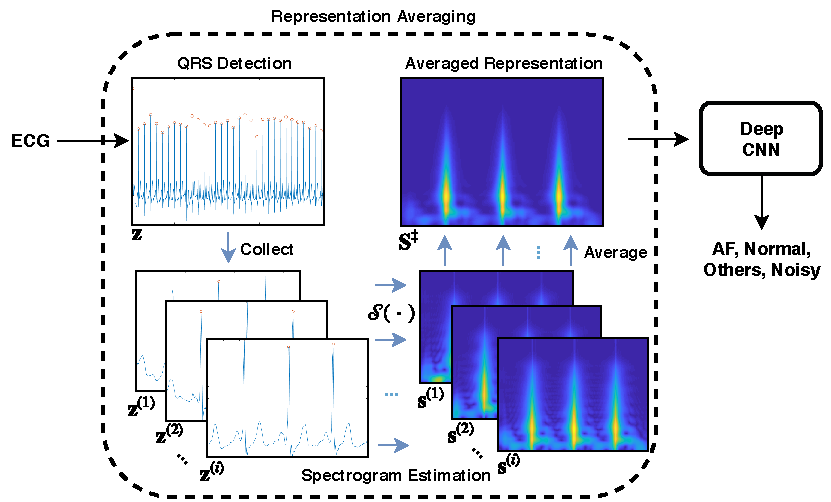
\includegraphics[scale=2]{figures/pre-processing}
\end{minipage}


\vspace{\sectionspace}
\section*{Spectro-Temporal ECG Analysis}

Different from classical transformation methods, we model the time varying spectrum with a state-space model and use Bayesian procedure (i.e., Kalman filter and smoother) for its estimation \cite{qi2002bayesian}, which does not need stationarity guarantee nor windowing. 

Recall that any periodic signal with fundamental frequency $f_0$ can be expanded into a Fourier series

\begin{equation}
z(t) = a_0 + \sum_{j=1}^{M} \left[ a_{j} \cos(2\pi \, j \, f_0 t) + b_{j} \sin(2\pi  \, j \, f_0 \, t) \right],
\label{equ:fourier_series}
\end{equation}

We assume that the coefficients depend on time, and we put a Gaussian process priors on them:
%
\begin{equation}
\begin{split}
a_j(t) &\sim \mathcal{GP}(0,k^a_j(t,t')), \\
b_j(t) &\sim \mathcal{GP}(0,k^b_j(t,t')).
\end{split}
\end{equation}

where the covariance functions are defined as: $k^a_j(t,t') = (s^a_j)^2 \, \exp( -\lambda^a_j \, | t - t' | )$ and $k^a_j(t,t') = (s^b_j)^2 \, \exp( -\lambda^b_j \, | t - t' | )$. The coefficients can be further represented in state-space, and discretized as \cite{Sarkka:2006}: 
%
%\begin{alignat*}{2}
%da_j &= -\lambda^a_j \, a_j \, dt + dW^a_j, \quad db_j &&= -\lambda^b_j \, b_j \, dt + dW^b_j \\
%a_j(t_k) &= \psi^a_{jk} \, a_j(t_{k-1}) + w^a_{jk}, \quad b_j(t_k) &&= \psi^b_{jk} \, b_j(t_{k-1}) + w^b_{jk},
%\end{alignat*}
%%
%where $W^a_j,W^b_j$ are Brownian motions with suitable diffusion coefficients $q^a_j,q^b_j$. We can also solve the equations at discrete time steps (see, e.g., \cite{Sarkka:2006}) as
%
\begin{equation}
\begin{split}
a_j(t_k) &= \psi^a_{jk} \, a_j(t_{k-1}) + w^a_{jk}, \\
b_j(t_k) &= \psi^b_{jk} \, b_j(t_{k-1}) + w^b_{jk}, \\
\end{split}
\label{eq:discdyn}
\end{equation}
%
where $\psi^a_{jk} = \exp(-\lambda^a_j \, (t_k - t_{k-1})), \psi^b_{jk} = \exp(-\lambda^b_j \, (t_k - t_{k-1}))$, $w^a_{jk} \sim \mathcal{N}(0,\Sigma^a_{jk}), w^b_{jk} \sim \mathcal{N}(0,\Sigma^b_{jk})$, $\Sigma^a_{jk} = q^a_j \, (1 - \exp(-2 \lambda^a_j \, (t_k - t_{k-1})))$, and $\Sigma^b_{jk} = q^b_j \, (1 - \exp(-2 \lambda^b_j \, (t_k - t_{k-1})))$. If we assume the input signal is noisy measurements from Fourier series \eqref{equ:fourier_series} and times $t_1,t_2,\ldots$, we can then model the time-varying system in state space, where state $\mathbf{x} = [a_{0}, a_{1}, ..., a_{M}, b_{1}, b_{2}, ..., b_{M}]^T$, and $\mathbf{H}_k = [1, \sin(2\pi f_0 t_k), \ldots, \sin(2\pi M \, f_0 \, t_k), \cos(2\pi f_0 t_k), \ldots, \cos(2\pi f_M t_j)]$, which gives $\mathbf{H}_k \mathbf{x}=z(t_k)$. The discrete-time dynamic model is written as:

\begin{equation}
\begin{split}
\mathbf{x}_k &= \mathbf{A}_{k} \mathbf{x}_{k-1} + \mathbf{q}_{k} \\
y_k &= \mathbf{H}_k \mathbf{x}_k + r_k.
\end{split}
\label{eq:dynmodel}
\end{equation}

where $\mathbf{A}_k$ contains the terms $\psi^a_{jk}$ and $\phi^b_{jk}$ on the diagonal and $ \mathbf{q}_{k} \sim \mathcal{N}(\mathbf{0},\mathbf{Q}_k)$ where $\mathbf{Q}_k$ contains the terms $\Sigma^a_{jk}$ and $\Sigma^b_{jk}$ on the diagonal.

% The end of the first column and the start of the second
\end{minipage} % no empty line before the next ``\begin''
\hspace{0.03\linewidth} % Middle margin
\begin{minipage}[t]{0.47\linewidth}
 % Paragraph indent
\Large

We could then perform exact Bayesian state estimation using Kalman filter and Rauch–Tung–Striebel (RTS) smoother, and define the spectro-temporal data matrix as:
\begin{equation}
[\mathbf{S}]_{j,k} = \sqrt{\hat{a}_{j}^2(t_k) + \hat{b}_{j}^2(t_k)}.
\label{eq:power_density}
\end{equation}

\begin{minipage}[c]{\linewidth}
	\centering
	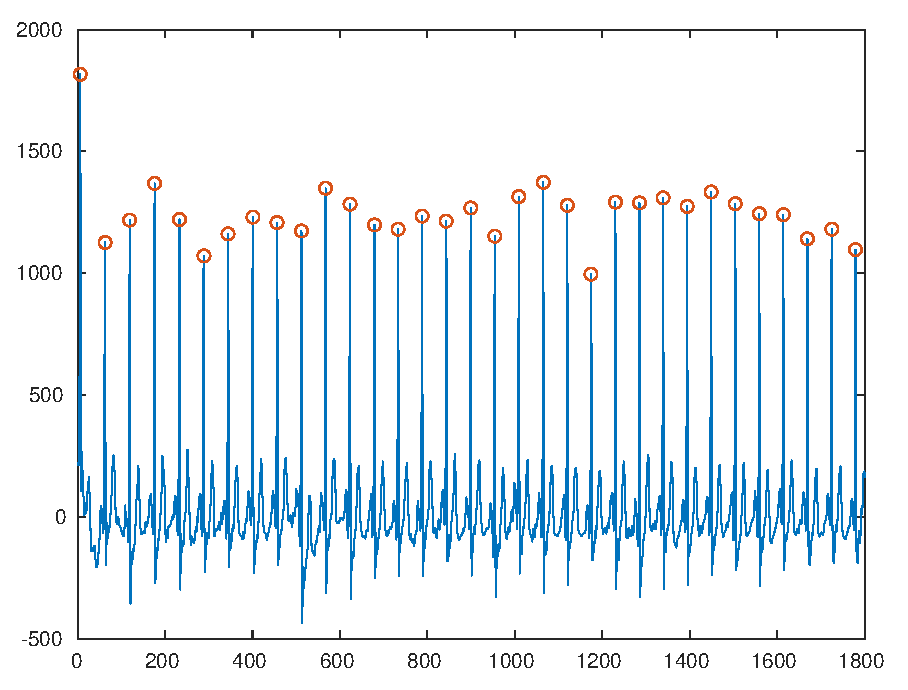
\includegraphics[width=0.22\linewidth]{figures/1012}
	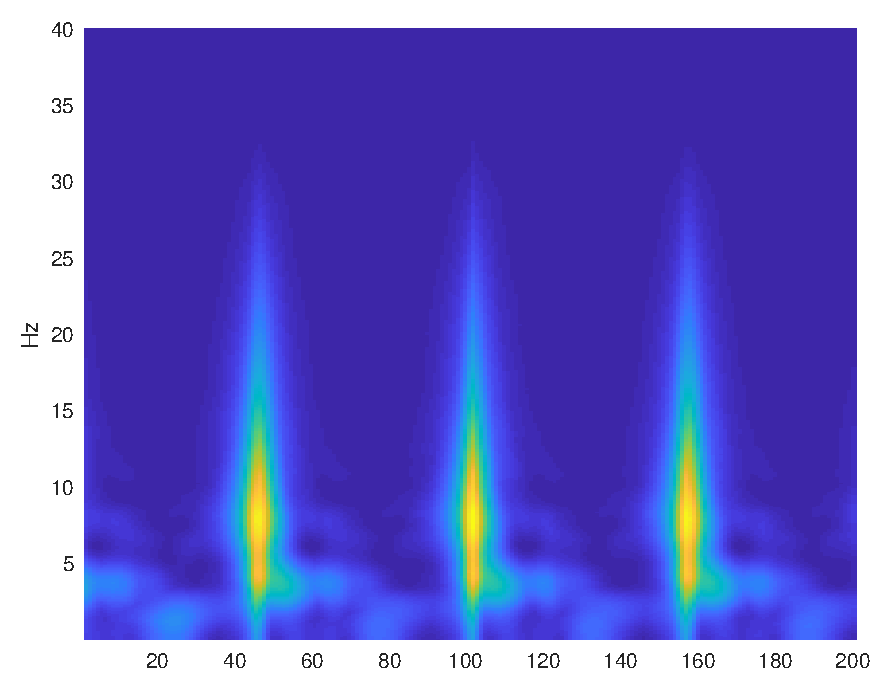
\includegraphics[width=0.22\linewidth]{figures/kalman-1012-smooth-large}
	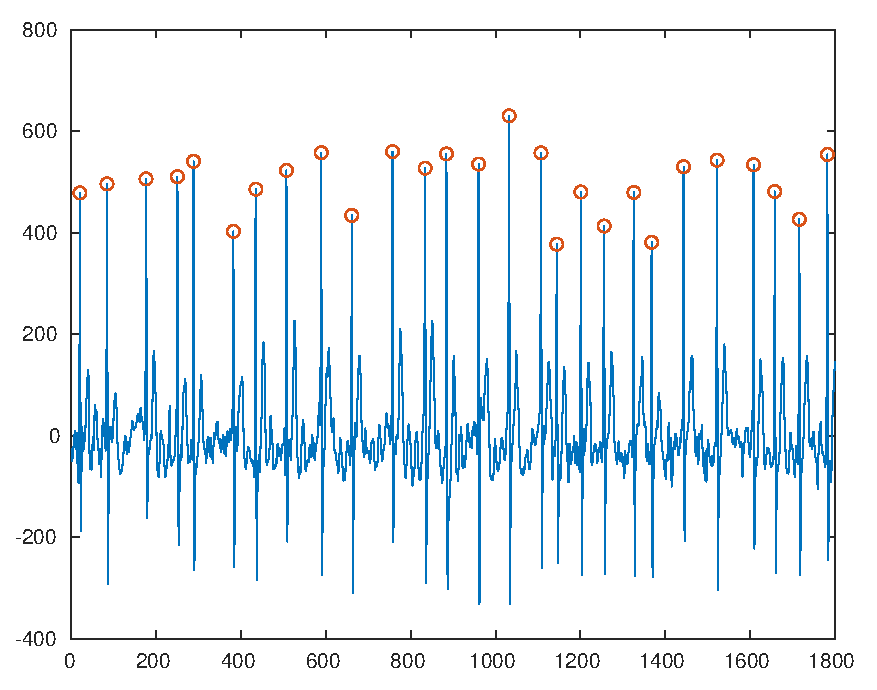
\includegraphics[width=0.22\linewidth]{figures/3246}
	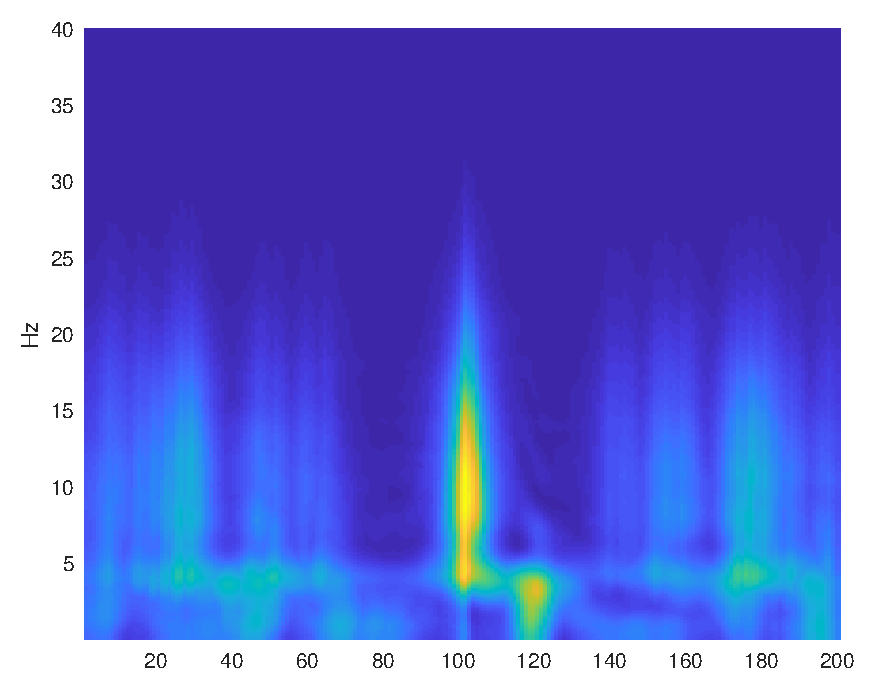
\includegraphics[width=0.22\linewidth]{figures/ave-af-3246}
	\\\small Normal (Rec.1012) \hspace{10cm} Atrial Fibrillation (Rec.3246)\\
	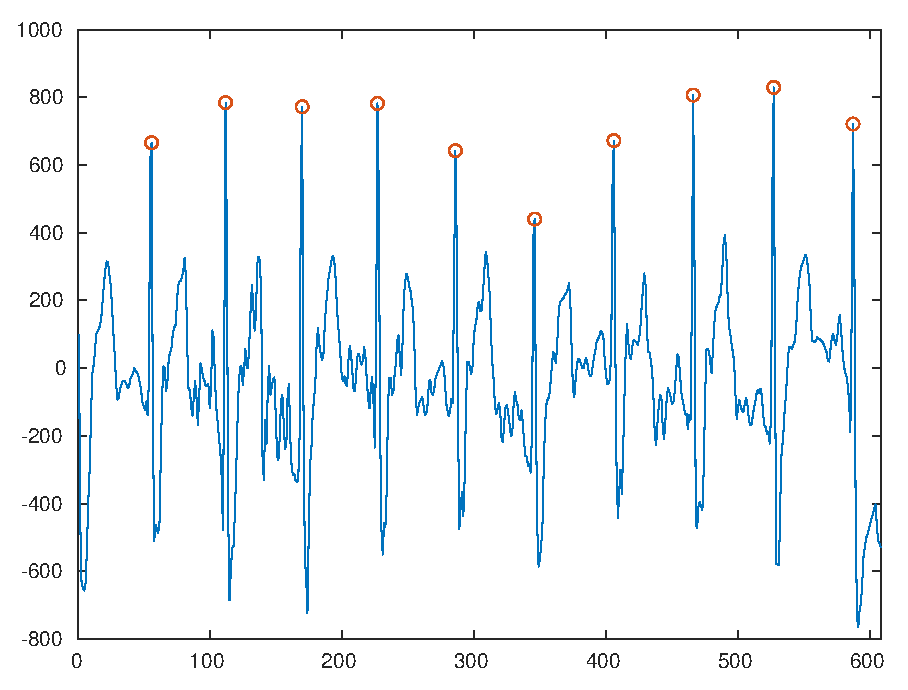
\includegraphics[width=0.22\linewidth]{figures/1037}
	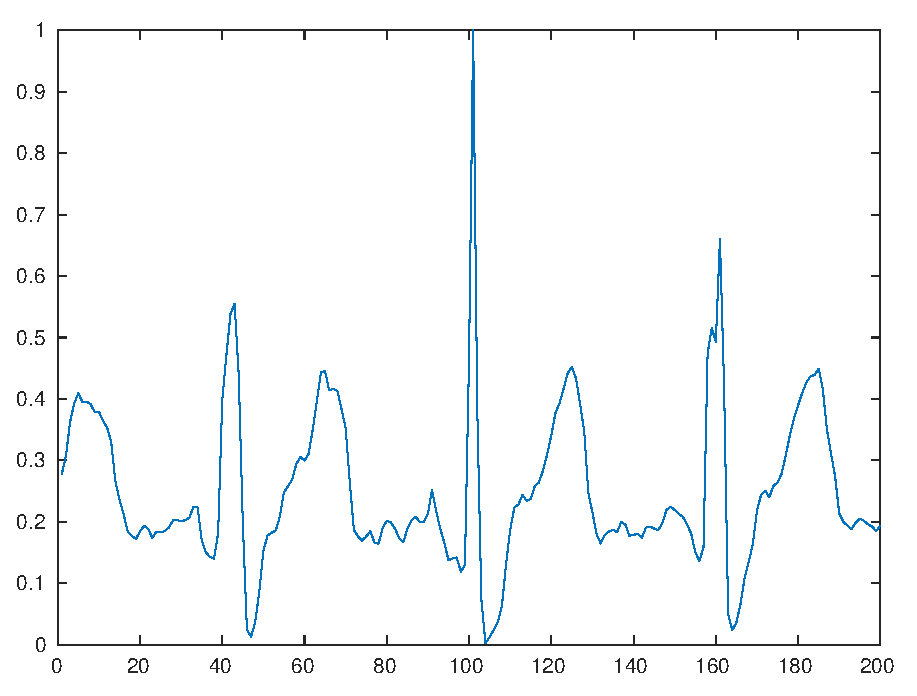
\includegraphics[width=0.22\linewidth]{figures/ave-other-1037}
	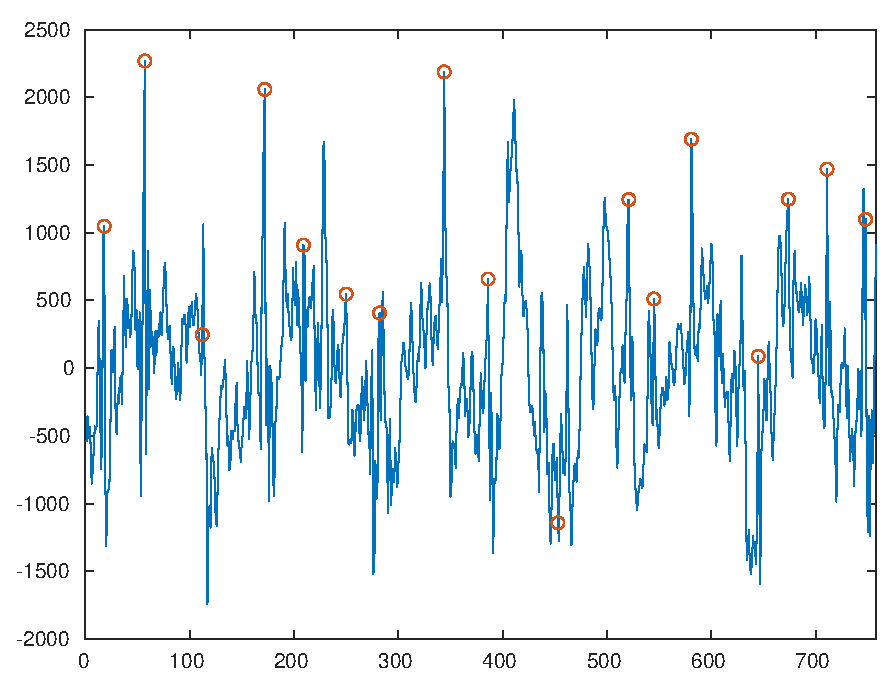
\includegraphics[width=0.22\linewidth]{figures/1006}
	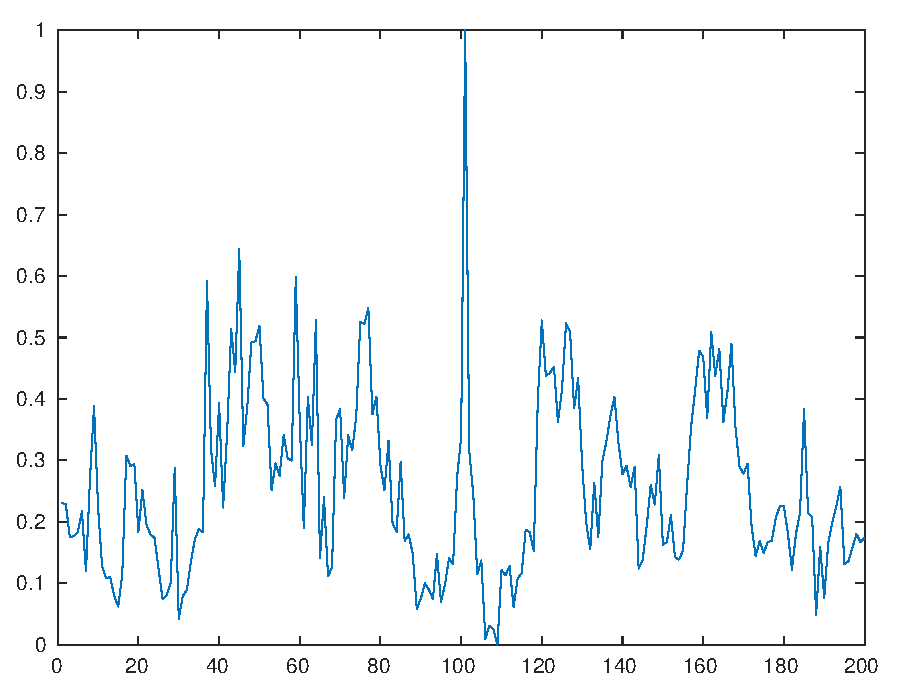
\includegraphics[width=0.22\linewidth]{figures/ave-noise-1006}
	\\Others (Rec.1037) \hspace{11cm} Noisy (Rec.1006)
\end{minipage}
\setlength{\parindent}{10mm}

In order to perform AF detection, we treat (\ref{eq:power_density}) as image data and train a DenseNet for ECG classification, where the structure is shown below:

\vspace{\figurespace}
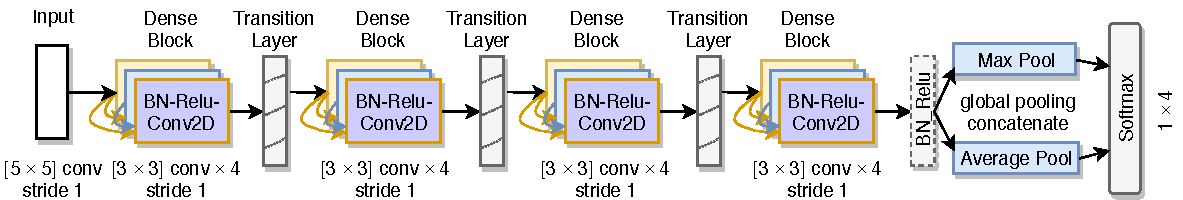
\includegraphics[scale=1.8]{figures/densely_banner}


\section*{Results}
The algorithm is performed on the PhysioNet/CinC 2017 dataset which contains 8528 short ECG recordings (9s to 60s) at 300Hz sampling rate. For model assessment, stratified 10-fold cross-validation and F1 metrics are adopted for evaluation. Below shows the confusion matrix and score:

\begin{minipage}[c]{\linewidth}
\setlength{\parindent}{0mm}
\vspace{\figurespace}
\centering
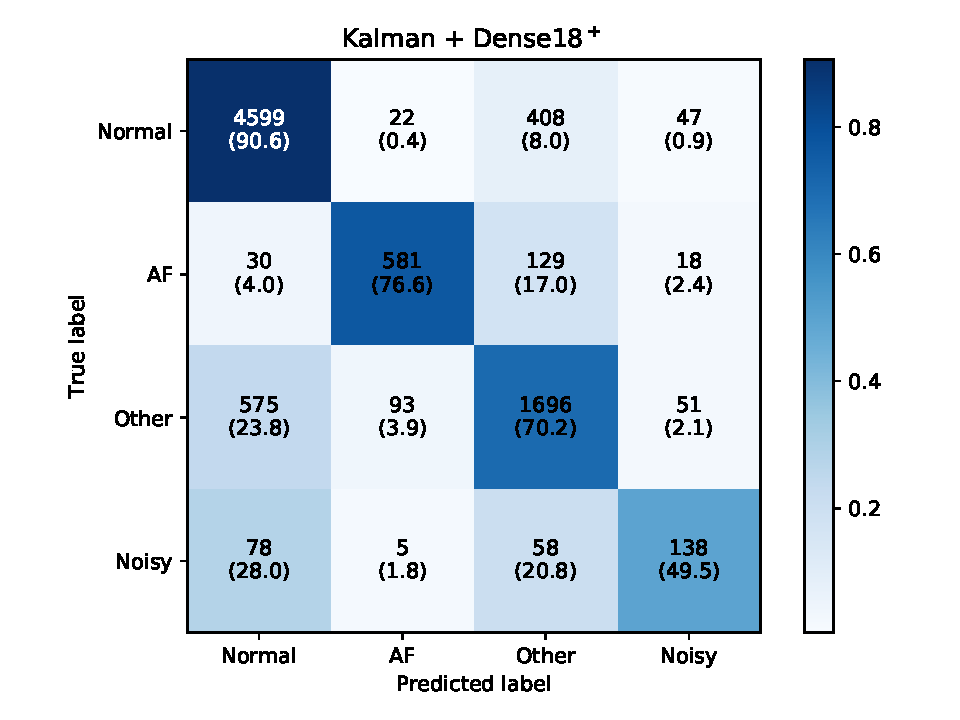
\includegraphics[width=0.24\linewidth,trim=1.15cm 0cm 1.2cm 0cm,clip]{figures/cm_kalman}
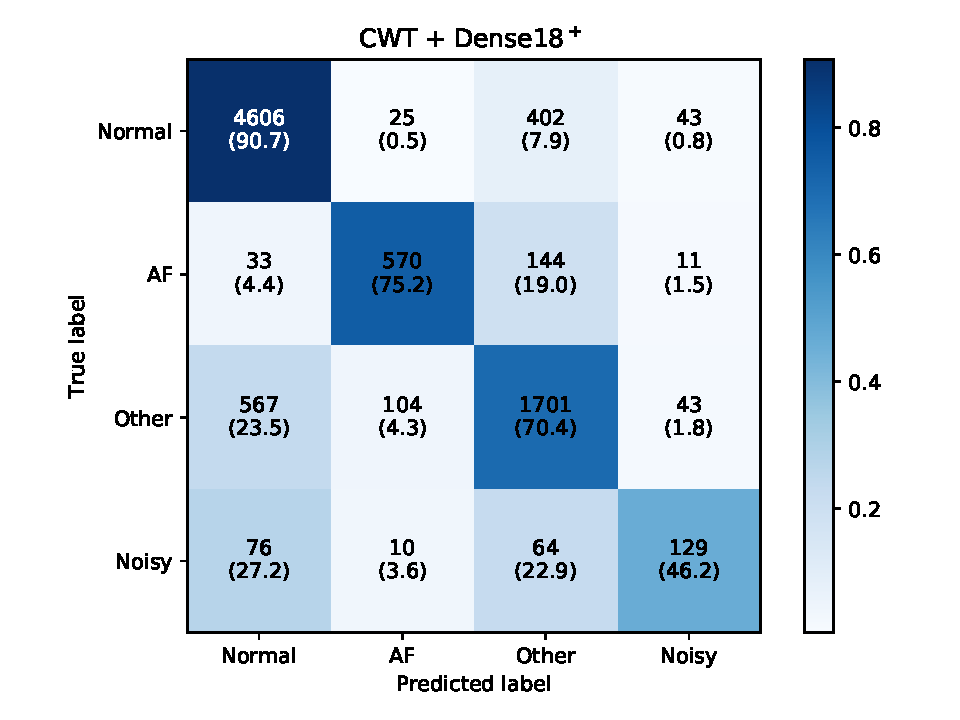
\includegraphics[width=0.24\linewidth,trim=1.15cm 0cm 1.2cm 0cm,clip]{figures/cm_cwt}
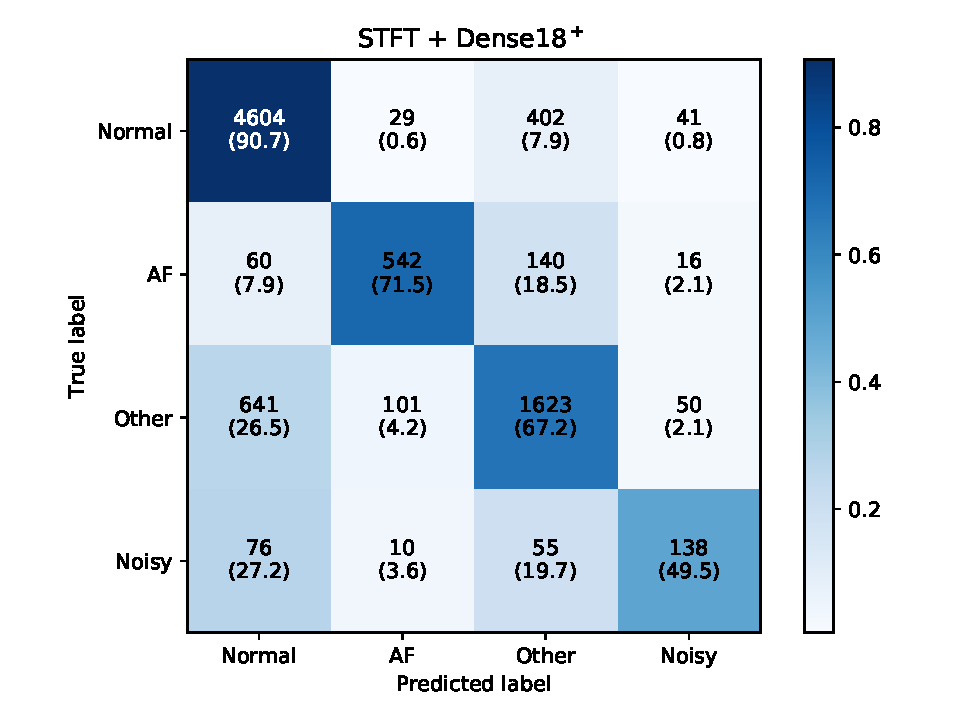
\includegraphics[width=0.24\linewidth,trim=1.15cm 0cm 1.2cm 0cm,clip]{figures/cm_stft}
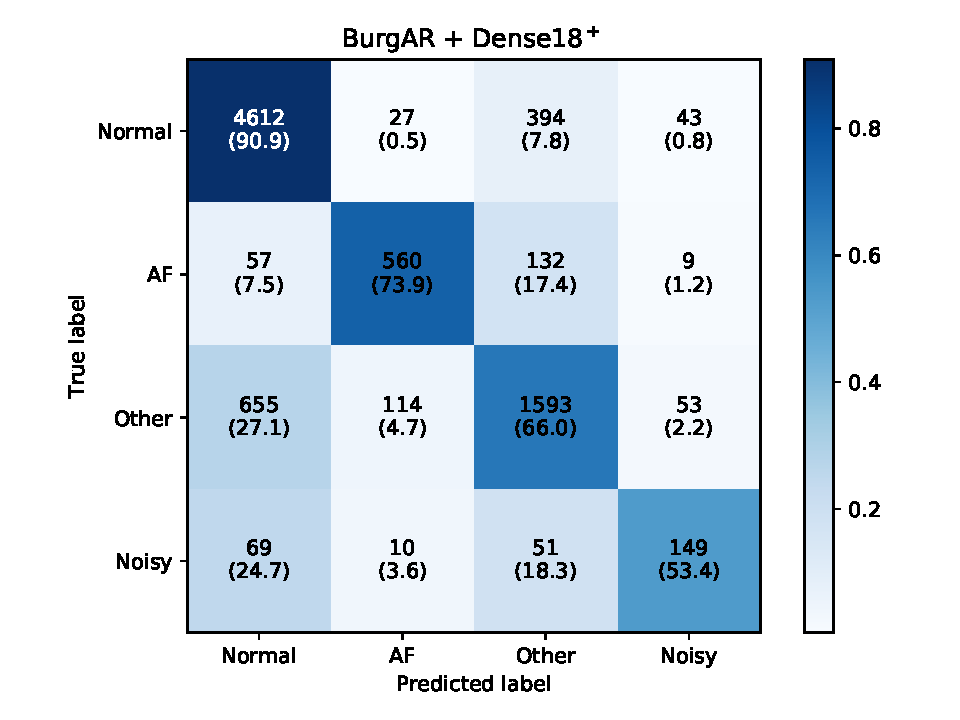
\includegraphics[width=0.24\linewidth,trim=1.15cm 0cm 1.2cm 0cm,clip]{figures/cm_pburg}
\large
Normalized confusion matrix on different methods.

\vspace{\figurespace}
\begin{tabular}{|l|l|c|c|c|c|c|c|c|}
	\hline
	& \multicolumn{1}{c|}{Methods}           & $F1_N$        & $F1_A$        & $F1_O$      & $F1_\sim$     & $F1_{overall}$  & $Std_{F1}$ & Precision \\ \hline
	(1) & STFT + Dense18$^+$                          & 88.06          & 75.23          & 70.03        & 52.67          & 77.79          & 1.41      & 79.38          \\ \hline
	(2) & CWT + Dense18$^+$                           & 88.77          & 78.08          & 71.79        & 53.25          & 79.55          & 1.39      & 80.73          \\ \hline
	(3) & BurgAR + Dense18$^+$                         & 88.11          & 76.24          & 69.49        & \textbf{55.91} & 77.95          & 1.51      & 79.23          \\ \hline
	(4) & Kalman + Dense18$^+$                        & \textbf{88.80} & \textbf{79.64} & \textbf{72.08}        & 51.78          & \textbf{80.17} & \textbf{1.06}      & \textbf{81.33} \\ \hline
	(5) & Kalman + Dense18                       & 88.16          & 76.61          & 70.81        & 49.21          & 78.53          & 1.14      & 80.02          \\ \hline
	(6) & Kalman + Res18                         & 87.19          & 74.98          & 68.31        & 47.01          & 76.83          & 1.08      & 78.04          \\ \hline
	(7) & Martin & 87.8            & 79.0            & 70.1 & 65.3   & 79.0            & N/A        & 81.2           \\ \hline
	(8) & Zhaohan                                & 87              & 80              & 68            & N/A             & 78              & N/A        & N/A             \\ \hline
\end{tabular}

\vspace{5mm}
Results from different spectrogram estimation methods and deep CNNs.
\end{minipage}

\vspace{\sectionspace}
\section*{Conclusion}
\setlength{\parindent}{10mm}
\begin{itemize}
	\item A new spectro-temporal analysis method is presented by assuming the time-varying Fourier coefficients of signal have Gaussian process priors. The solution is in linear state-space and state estimation is performed by Bayesian Kalman filter/smoother. 
	\item We combine this spectro-temporal method with deep CNNs for ECG classification. The proposed method outperforms other time-frequency analysis methods (i.e., STFT, CWT, and BurgAR) and provides the classification performance of 80.2\% for overall F1 score. 
\end{itemize}

\begin{textblock}{24}(57,115)
	\large \textbf{Contact: Zheng Zhao (zheng.zhao@aalto.fi)}
\end{textblock}

%{\tiny % % Bibliography text size begins...
{\footnotesize % % Bibliography text size begins...

\bibliographystyle{IEEEtran}
\bibliography{refs}

} % <- bibliography text size ends

\end{minipage}
\end{minipage} % minipage for the two columns (minipages)





% \vfill % Fill the free space until the footer minipages


%\begin{minipage}{0.95\linewidth} % Minipages for the footers
%
%
%\footnotesize % Text size for footers
%
%
%\begin{minipage}[t]{0.47\linewidth}% Footer #1
%\vspace{0pt}
%
%\textsf{\textbf{Department of Radio Science and Engineering / SMARAD Centre of Excellence\\
%School of Electrical Engineering\\
%Aalto University, Finland}}
%
%\end{minipage} % No empty line before the second begin!
%\hspace{0.03\linewidth}
%\begin{minipage}[t]{0.47\linewidth} % Footer #2
%\vspace{0pt}
%
%\textsf{\textbf{Contact information for comments \& improvement ideas: Antti Karilainen\\
%Email: antti.karilainen@aalto.fi\\
%Version 0.1g}}
%\end{minipage}
%
%
%
%\end{minipage}




% \vspace*{0.03\linewidth} % Increase the bottom margins



\end{document}
